\section{Experiments}
\subsection{Dataset}
We collected blah blah videos from YouTube and did blah blah... All numbers etc. These are recipes, 5 of them are evaluation set and labelled temporally and labels are matched.
\subsection{Baselines}
We compare against BP-HMM-O with local feauters and HMM with Semantic Features, HMM with local features, HMM with CNN feautes...
\subsection{Qualitative Results}
\begin{figure}
  \begin{subfigure}[b]{0.5\textwidth}
  \includegraphics[width=\textwidth]{act_gt}
  \caption{Ground Truth Activity Labels}
  \end{subfigure}
  \begin{subfigure}[b]{0.5\textwidth}
  \includegraphics[width=\textwidth]{act_our}
  \caption{Activity Labels extracted by Our Method}
  \end{subfigure}

\begin{subfigure}[b]{0.5\textwidth}
\begin{subfigure}[b]{0.5\textwidth}
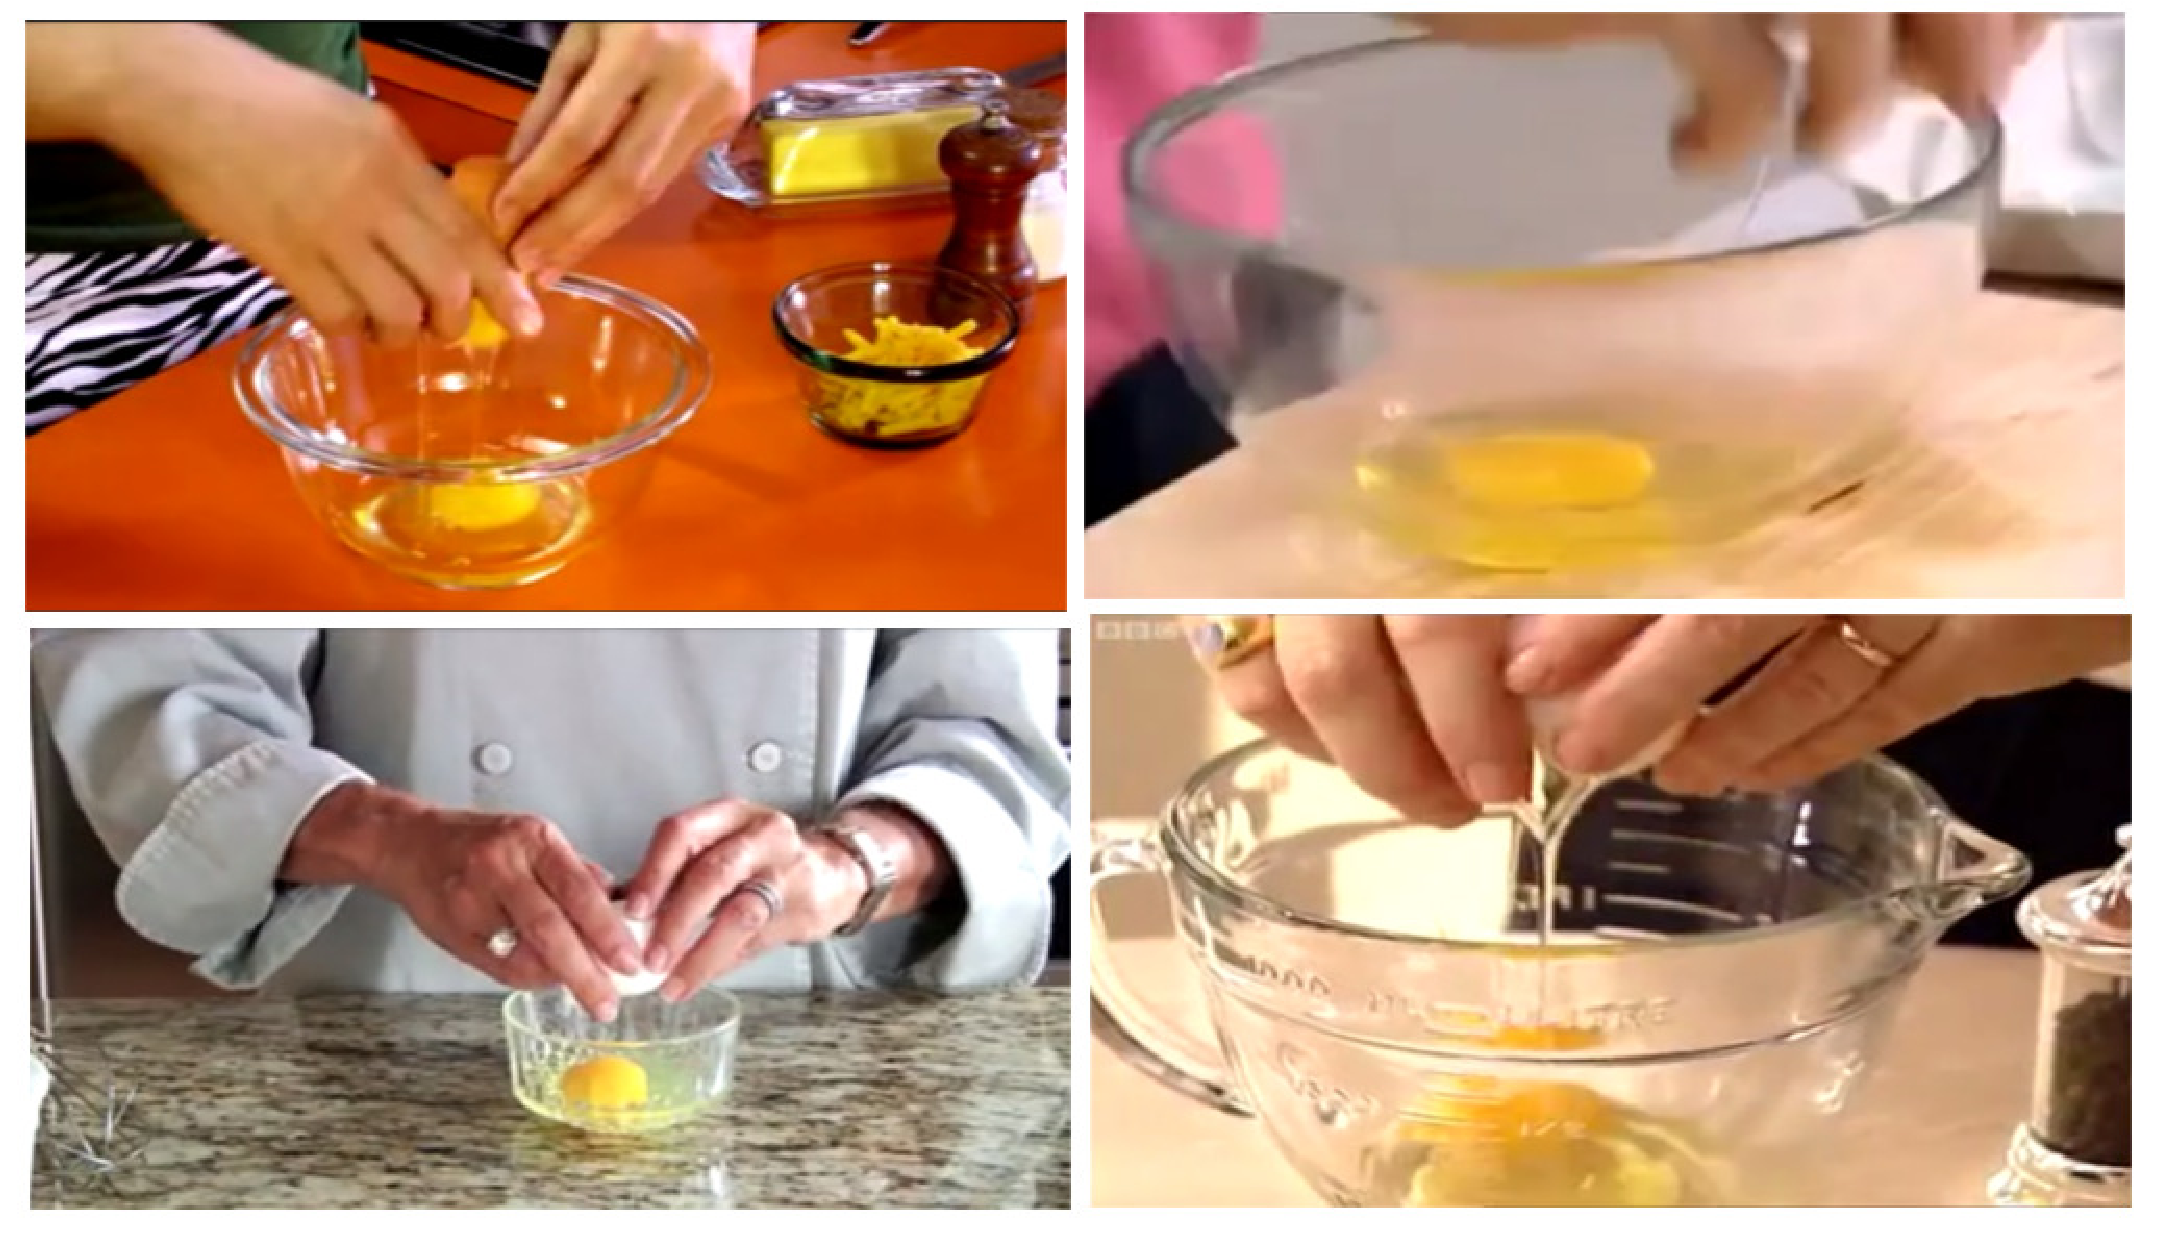
\includegraphics[width=\textwidth]{cred}
\color[HTML]{FF3800}{Crack the eggs one at a time into a bowl.}
\end{subfigure}~
\begin{subfigure}[b]{0.5\textwidth}
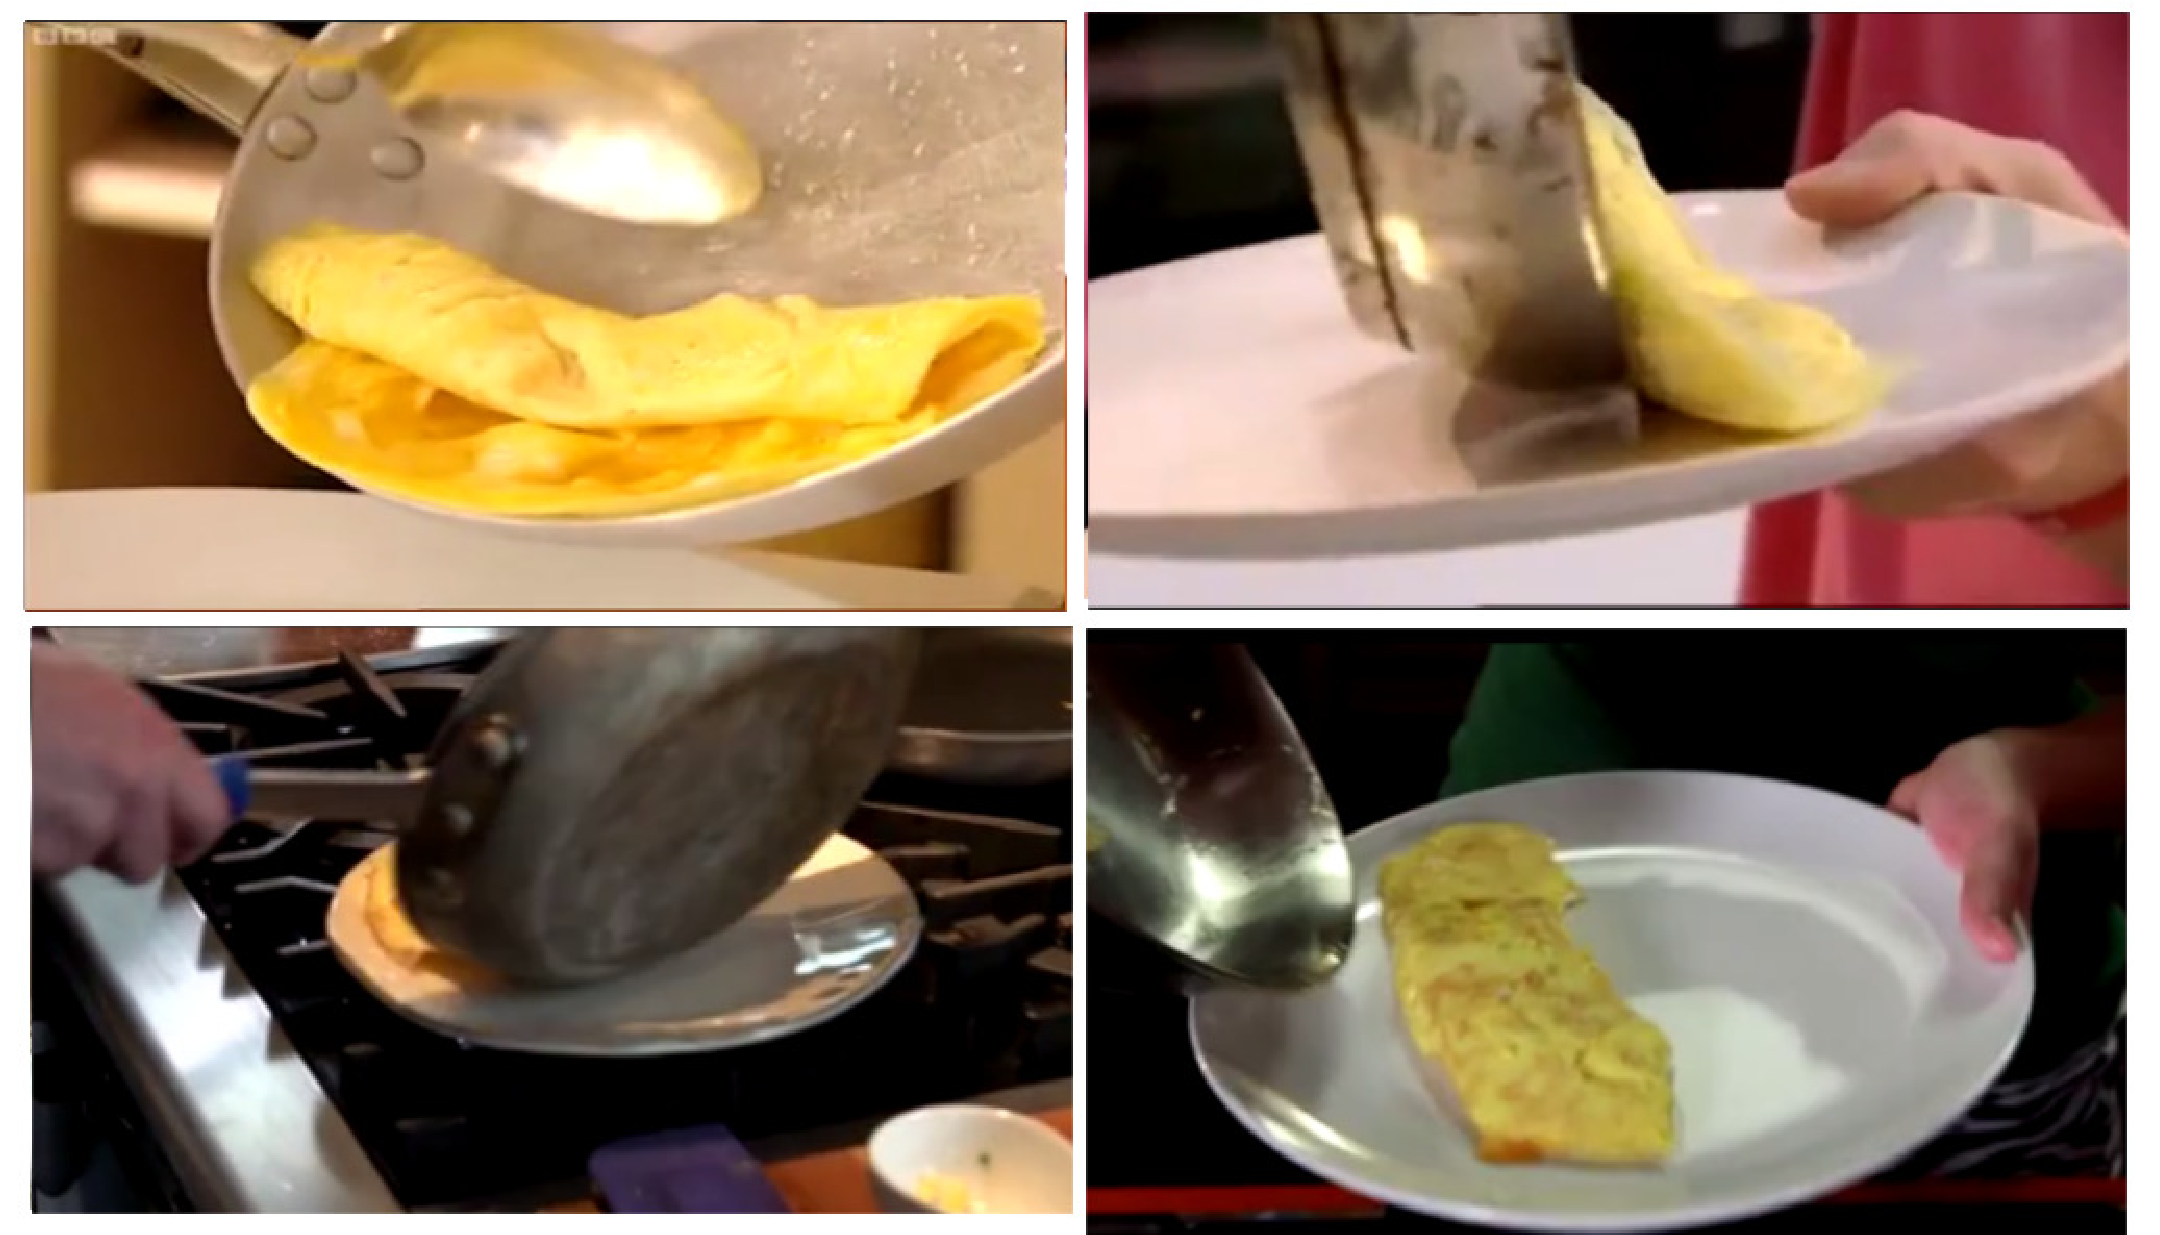
\includegraphics[width=\textwidth]{cyan}
\color[HTML]{00FFED}{Remove the omelette onto a plate.}
\end{subfigure}


\begin{subfigure}[b]{0.5\textwidth}
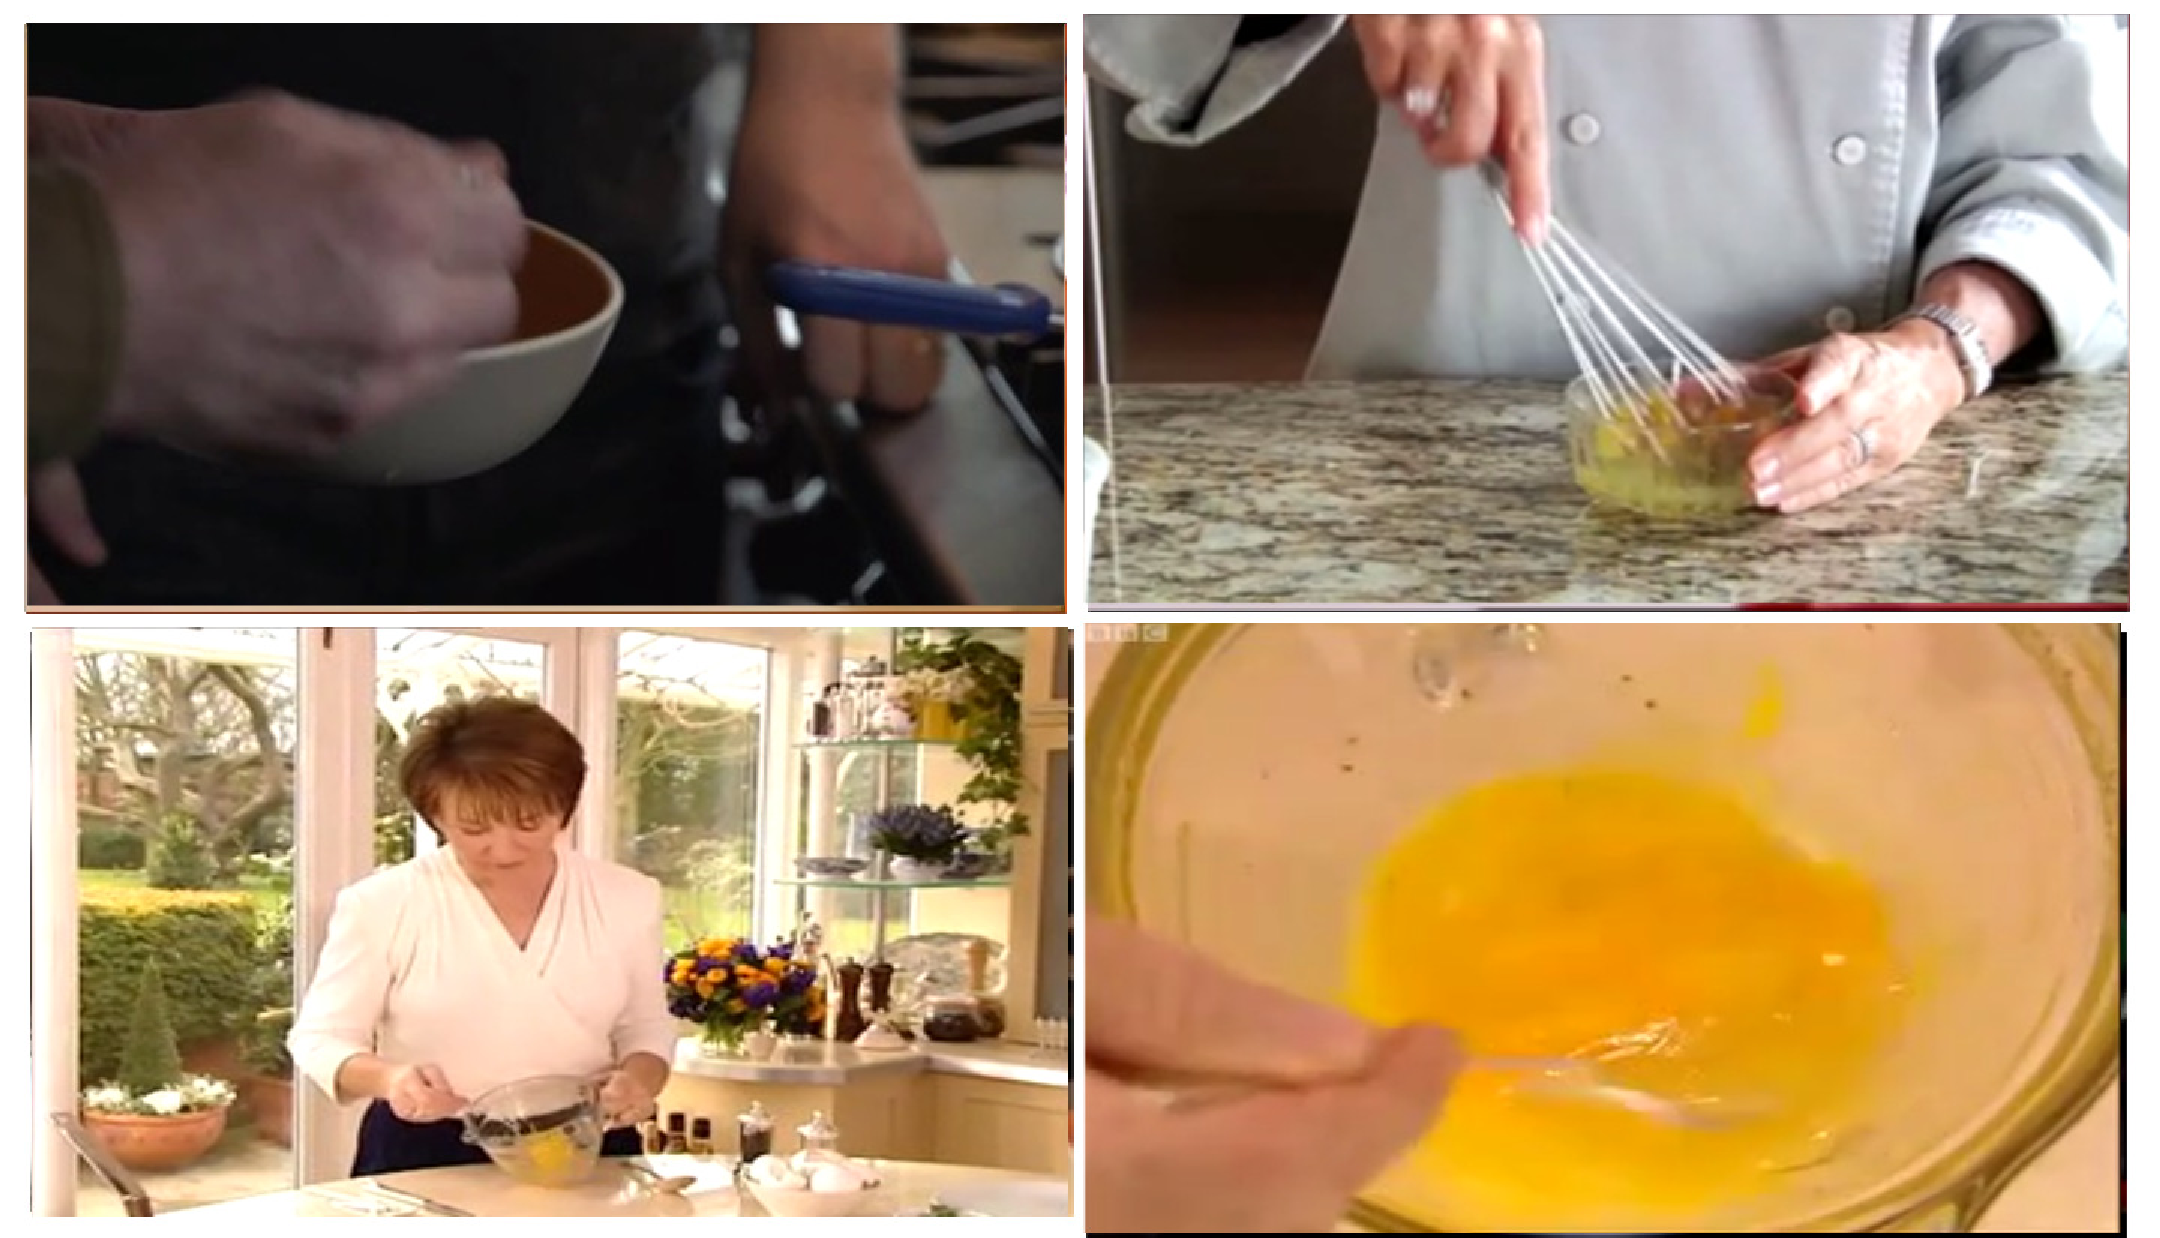
\includegraphics[width=\textwidth]{corange}
\color[HTML]{FF9900}{You can either use a fork or wire whisk to beat the eggs into a bowl.}
\end{subfigure}~
\begin{subfigure}[b]{0.5\textwidth}
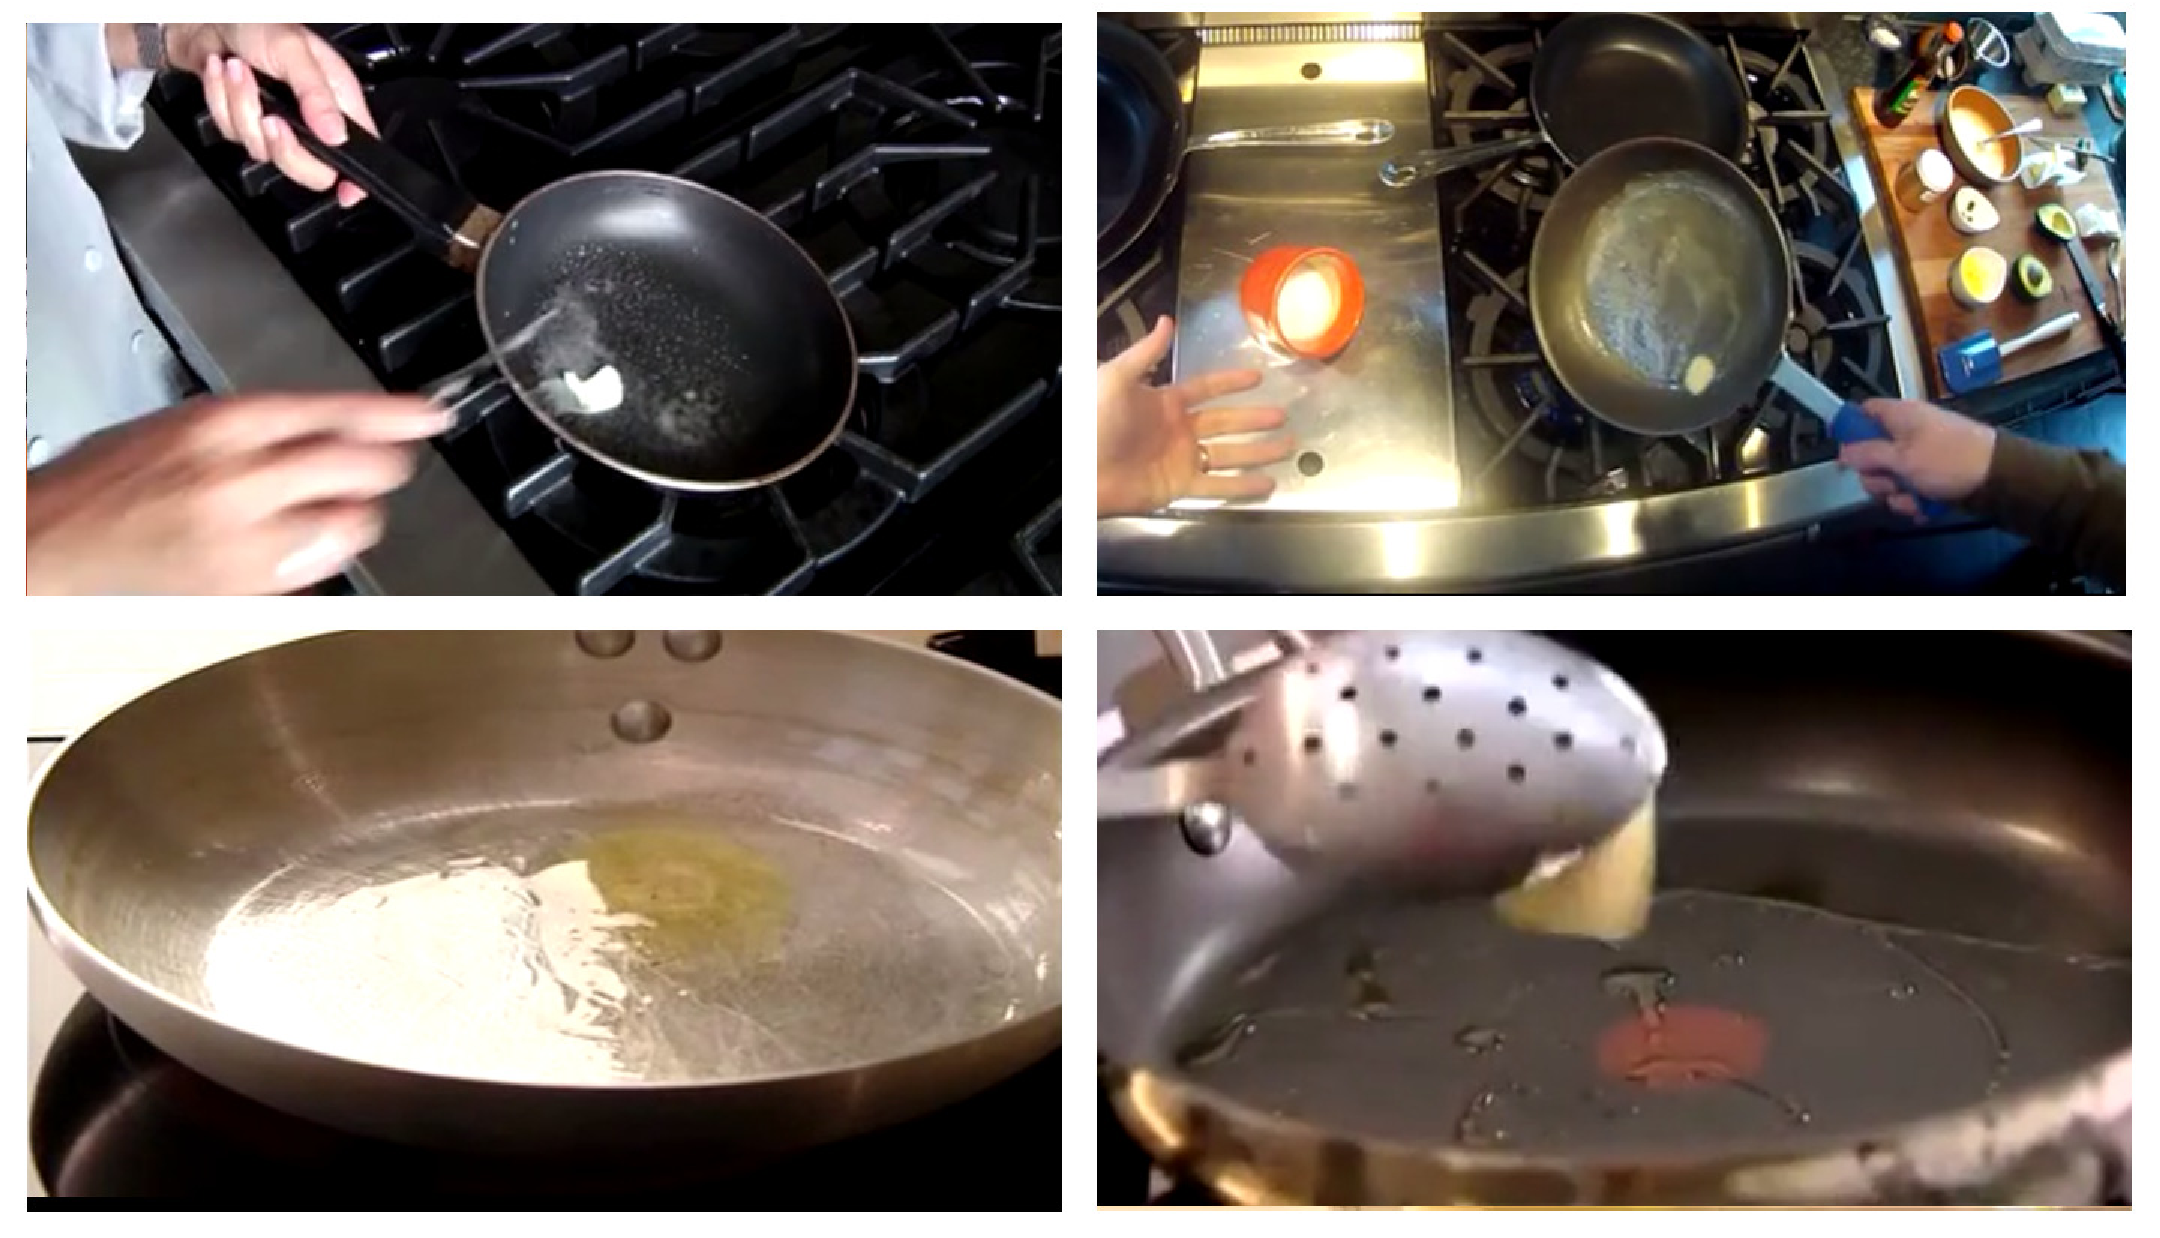
\includegraphics[width=\textwidth]{cgreen}
\color[HTML]{9DFF00}{Eggs cook quickly, so make sure the pan gets very hot first; the butter melt completely.}
\end{subfigure}



\caption{Sample images and the automatically generated captions for some of the clusters.}
\end{subfigure}

\end{figure}
\subsection{Accuracy over Activity Detection}
\subsection{Accuracy over Activity Learning}
